\documentclass[11pt,a4paper]{article}
\usepackage[T1]{fontenc}\usepackage{mathptmx}\usepackage[margin=25mm]{geometry}\usepackage{graphicx}
\pagestyle{empty}
\begin{document}
\noindent\textbf{Graphical Table of Contents}\par\bigskip
\noindent\textbf{Testing What a Score Measures: Validating and Repairing the Calibration Scores of a Personal Decision Analytics System}\par\medskip
\noindent Shakil Ur Rehman*\par\bigskip
\noindent\begin{minipage}[t]{50mm}\vspace{0pt}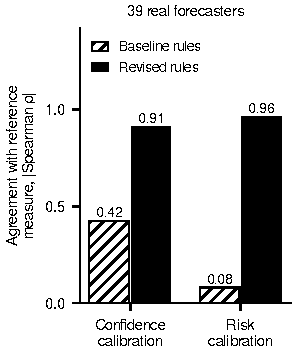
\includegraphics[width=50mm,height=60mm,keepaspectratio]{GTOC_figure.pdf}\end{minipage}\hfill
\begin{minipage}[t]{0.58\textwidth}\vspace{0pt}
Two of four baseline scores of a personal decision-analytics application computed their formulas correctly yet did not measure what their names claimed. Metamorphic relations derived from score names, simulation with known miscalibration and a replay of 4,793 real forecasts exposed both defects without a user study, alongside a race condition, unescaped output and an N+1 query pattern. The revised rules raise agreement with standard calibration measures from $|\rho| = 0.42$ and $0.08$ to $0.91$ and $0.96$.
\end{minipage}\par\bigskip
\noindent{\small *Corresponding author}
\end{document}
